%%%%%%%%%%%%%%%%%%%%%%%%%%%%%%%%%
% ammana.es | Manual de cliente %
%                               %
%  Made with ❤️  by NoLegalTech  %
%%%%%%%%%%%%%%%%%%%%%%%%%%%%%%%%%

\documentclass[12pt, spanish]{article}

\usepackage{geometry}
\geometry{a4paper}

\usepackage{graphicx}
\graphicspath{{img/}}

\usepackage{adjustbox}

\usepackage{float}
\usepackage{wrapfig}

\usepackage[spanish]{babel}
\selectlanguage{spanish}

\usepackage[utf8]{inputenc}

\usepackage{enumitem}

\linespread{1.2}

\setlength{\parindent}{2em}
\setlength{\parskip}{1em}

\usepackage{concmath}
\usepackage[T1]{fontenc}

\usepackage{fancyhdr}

\fancyhf{}
\fancyhead[L]{
\includegraphics[height=5.0mm]{logo}}

\newlist{steps}{enumerate}{1}
\setlist[steps]{label={\arabic*)}}

\setlength{\headheight}{7.50mm}
\pagestyle{fancy}

%----------------------------------------------------------------------------------------

\begin{document}

%----------------------------------------------------------------------------------------

\begin{titlepage}

    \newcommand { \HRule } { \rule {\linewidth} {0.5mm} }

    \center

    \textsc {\LARGE ammana.es} \\ [1.5cm]

    \HRule \\ [0.4cm]

    { \huge \bfseries Manual del administrador } \\ [0.4cm]

    \HRule \\ [1.5cm]

    { \large \today } \\ [3cm]

    \vfill

\end{titlepage}

%----------------------------------------------------------------------------------------

\tableofcontents

\newpage

%----------------------------------------------------------------------------------------
\section{Introducción}

    \textbf{ammana.es} funciona de forma prácticamente autónoma y los clientes pueden
    comprar y descargar protocolos sin intervención del administrador. La única
    excepción es cuando algún cliente paga por transferencia bancaria, en cuyo
    caso el pago debe ser marcado como cobrado de forma manual para que el cliente
    pueda descargarse el protocolo.

    Por otro lado, el panel de administración de \textbf{ammana.es}, junto con los de \textbf{Paypal} y
    \textbf{Quaderno}, dan acceso al administrador a la lista de clientes, facturas, pedidos, etc
    para su consulta, bien por curiosidad bien para ofrecer soporte a un cliente..

    Es decir, las funciones del administrador son 2:

    \begin{steps}
      \item Marcar como cobrados los pedidos que han sido pagados por transferencia
      \item Acceder a la información de clientes y facturas
    \end{steps}

%----------------------------------------------------------------------------------------
\section{Acceso al panel de administración}

Para acceder al panel de administración, simplemente debes hacer login con las credenciales
del usuario, administrador. Es decir:

\begin{steps}
    \item Click en ``Identificarse'':

        \medskip
        \begin{minipage}[t]{\linewidth}
        \raggedright
        \adjustbox{valign=t}{%
            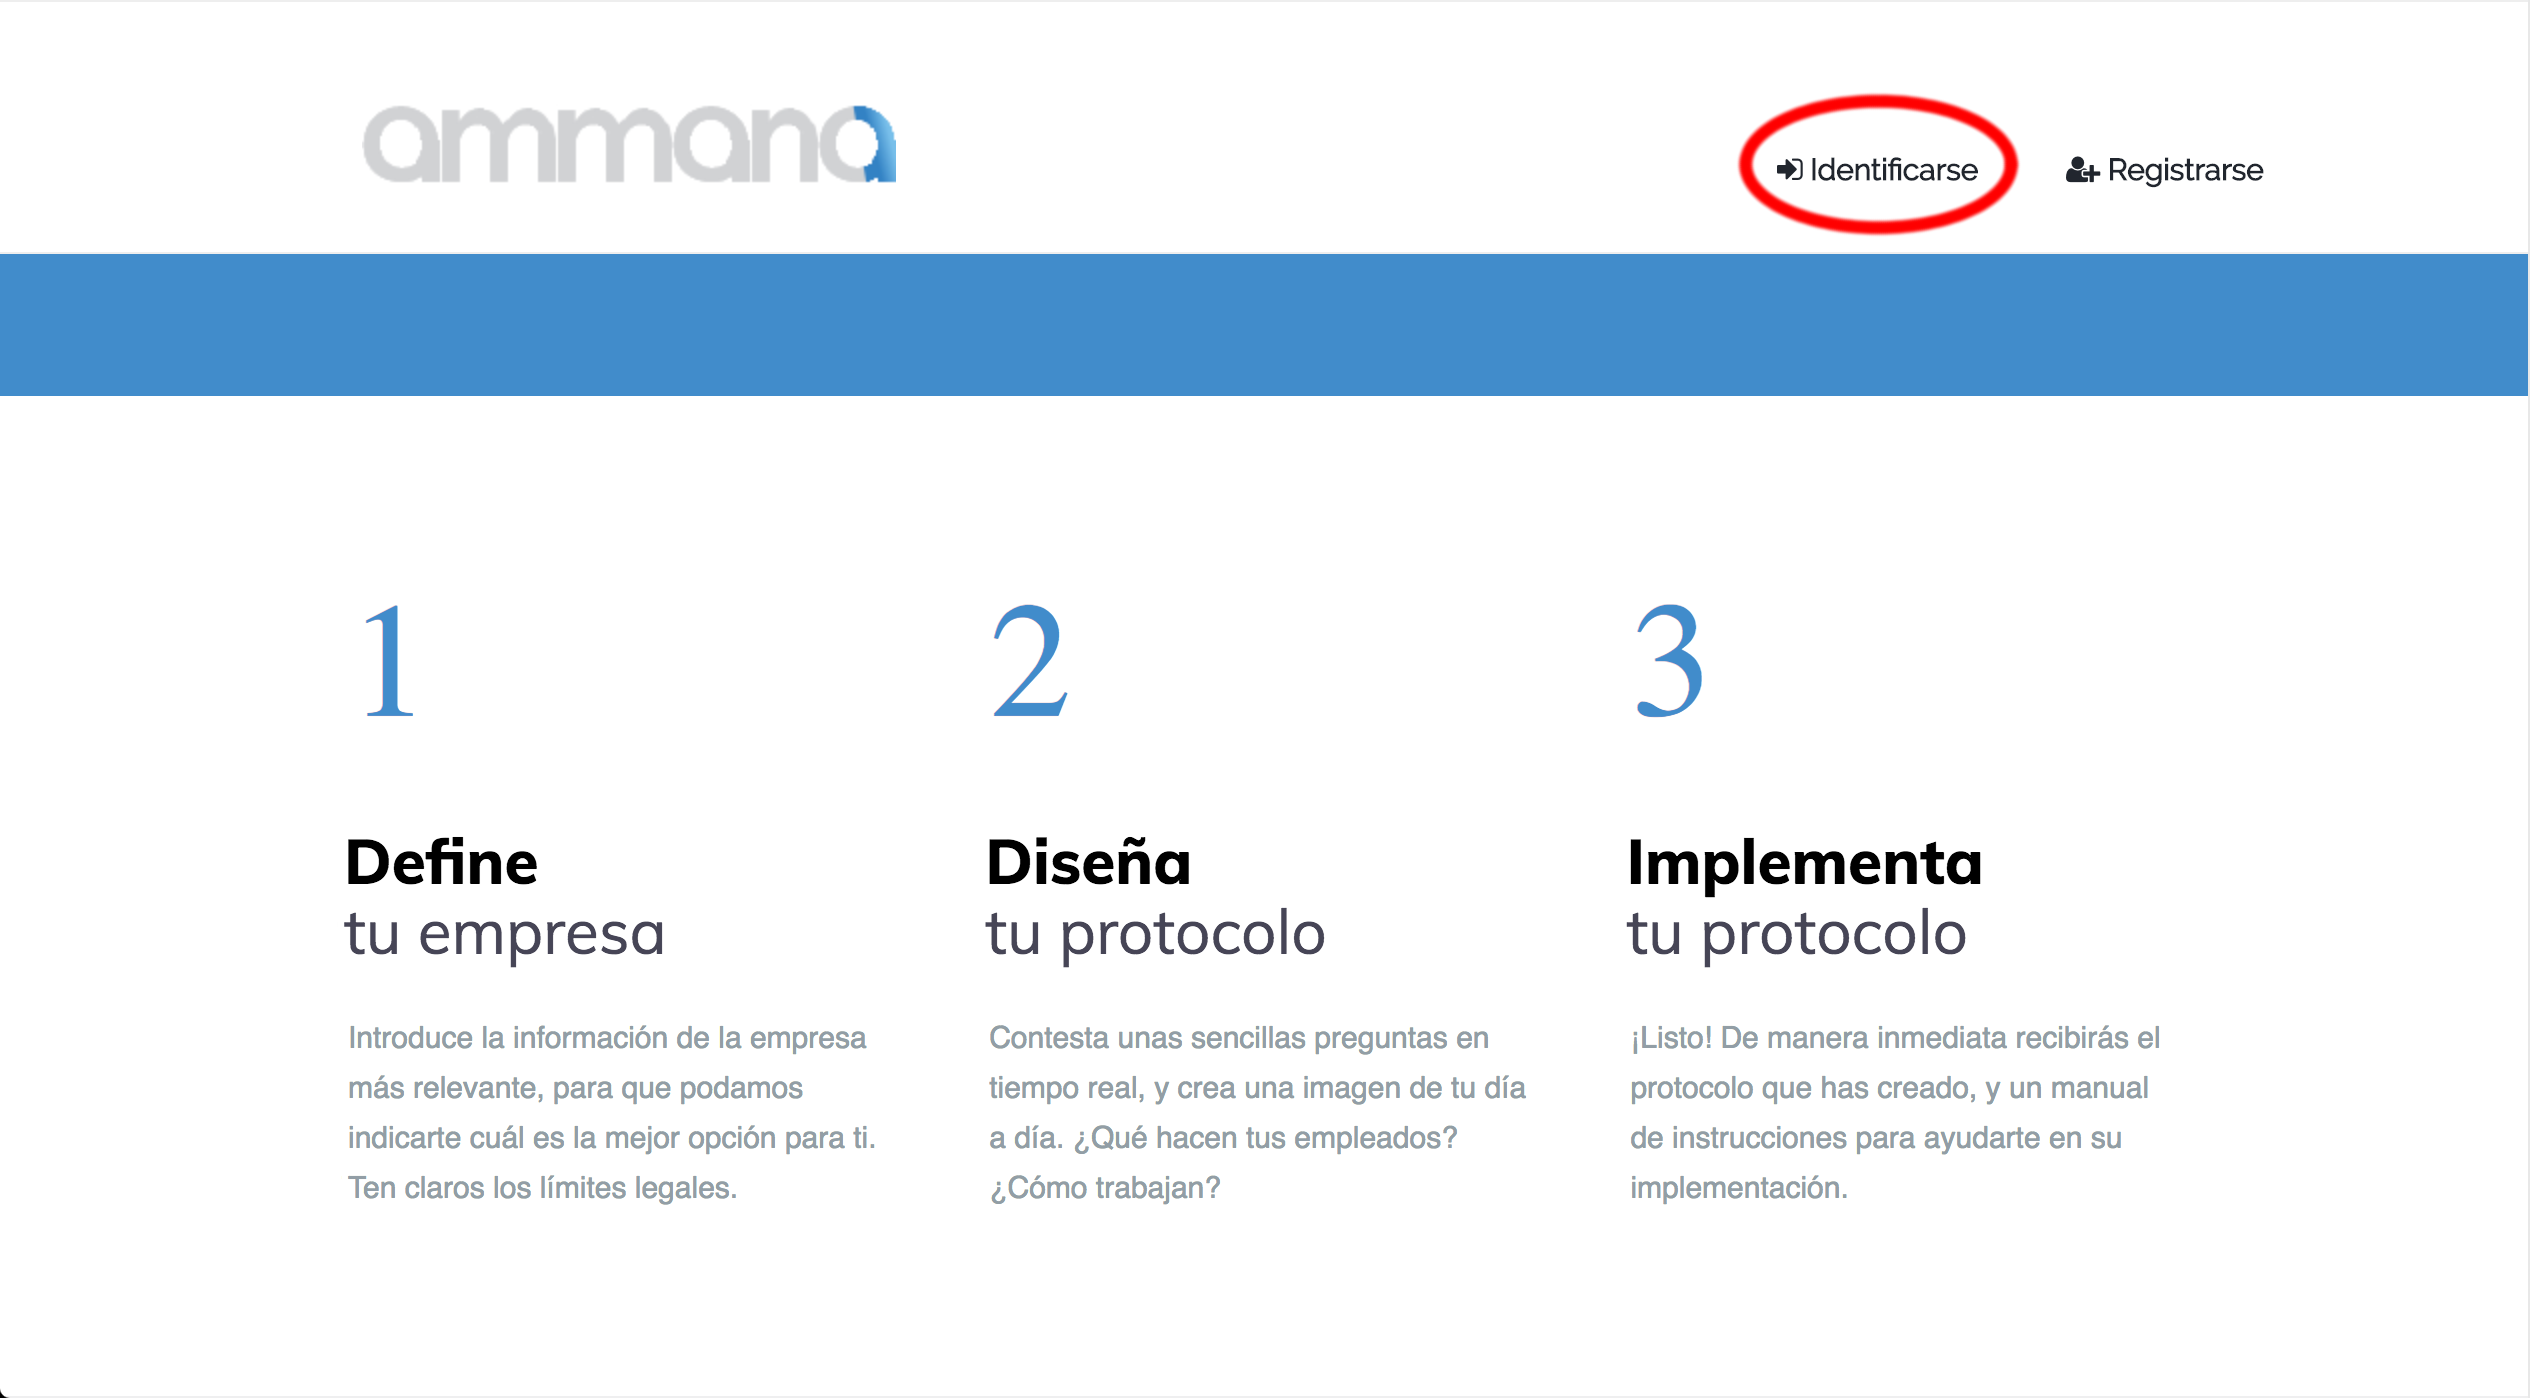
\includegraphics[width=1\linewidth]{login_button.png}%
        }
    \end{minipage}
    \item Introducir email y contraseña en el formulario de login:

        \medskip
        \begin{minipage}[t]{\linewidth}
        \raggedright
        \adjustbox{valign=t}{%
            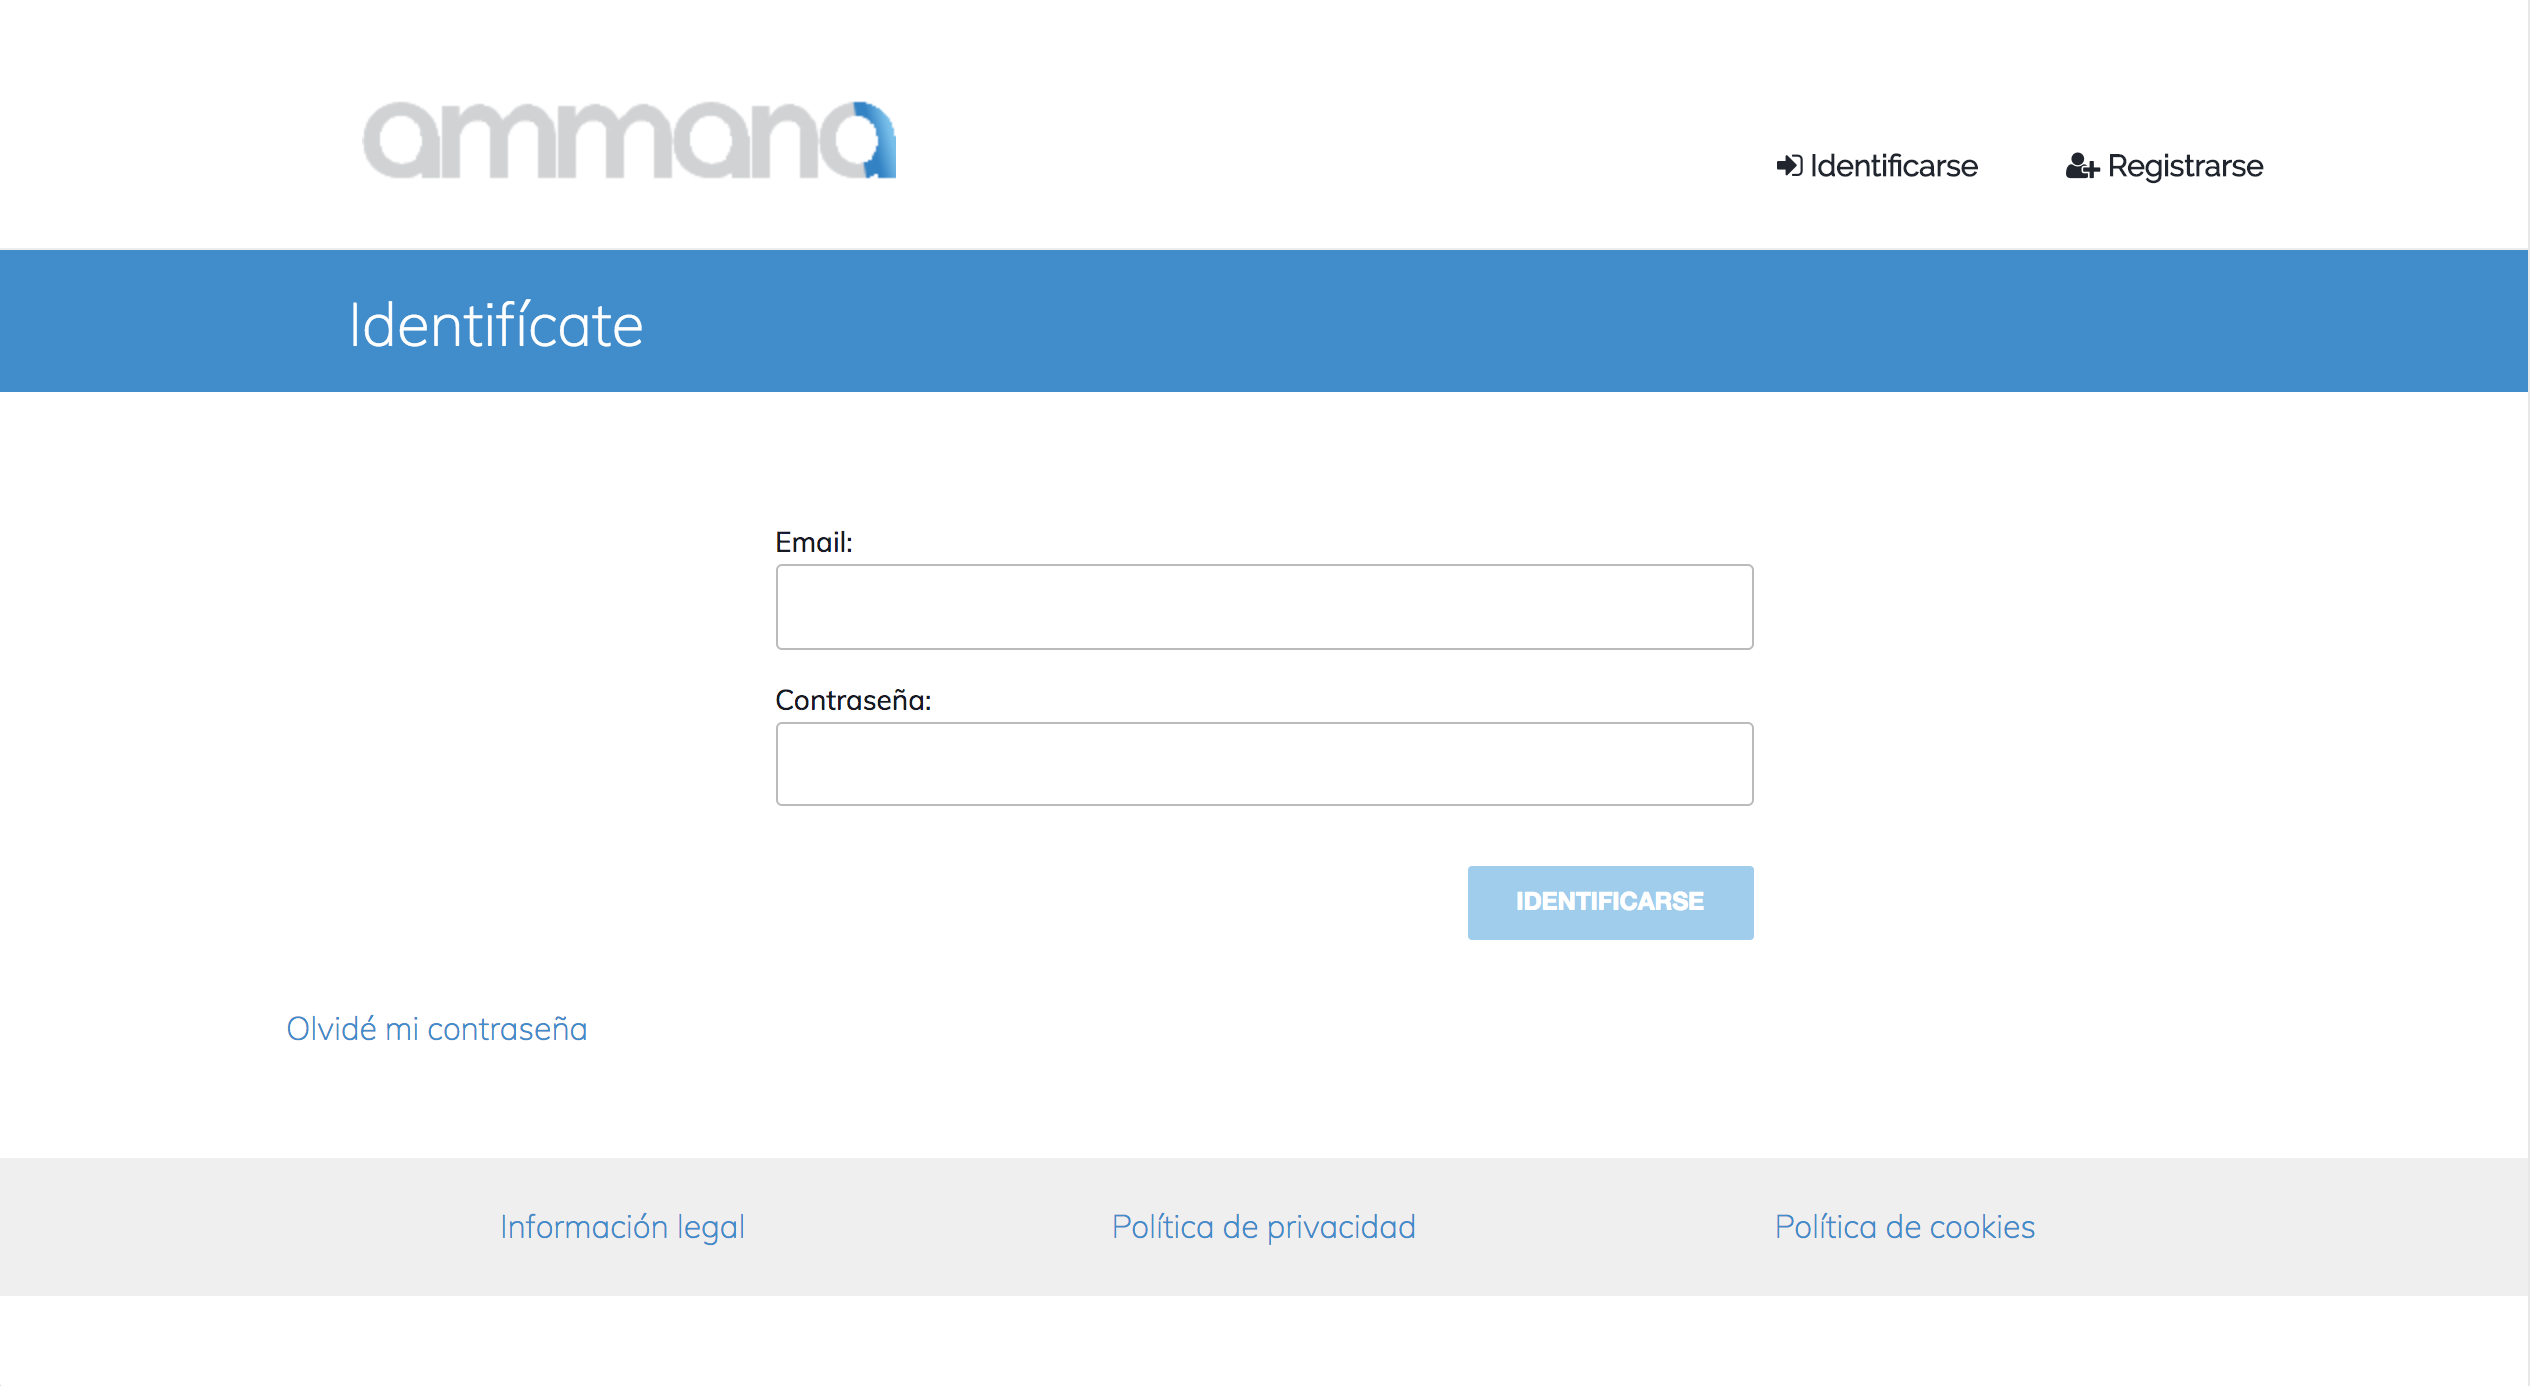
\includegraphics[width=1\linewidth]{login_form.png}%
        }
    \end{minipage}
\end{steps}

%------------------------------------------------

\subsection{Subsection 2} % Sub-section

Lorem ipsum

%------------------------------------------------

\subsubsection{Subsubsection 1} % Sub-sub-section

Lorem ipsum...

\begin{figure}[H] % Example image
\center{
\includegraphics[width=0.5\linewidth]{placeholder}}
\caption{Example image.}
\label{fig:speciation}
\end{figure}

%------------------------------------------------

\subsubsection{Subsubsection 2} % Sub-sub-section

Lorem ipsum...

%----------------------------------------------------------------------------------------
%	MAJOR SECTION 1
%----------------------------------------------------------------------------------------

\section{Content Section} % Major section

Lorem ipsum...

%------------------------------------------------

\subsection{Subsection 1} % Sub-section

\subsubsection{Subsubsection 1} % Sub-sub-section

Lorem ipsum...

%------------------------------------------------

\subsubsection{Subsubsection 2} % Sub-sub-section

Lorem ipsum...
\begin{wrapfigure}{l}{0.4\textwidth} % Inline image example
  \begin{center}
    
\includegraphics[width=0.38\textwidth]{fish}
  \end{center}
  \caption{Fish}
\end{wrapfigure}
Lorem ipsum...

%------------------------------------------------

\subsubsection{Subsubsection 3} % Sub-sub-section

\begin{description} % Numbered list example

\item[First] \hfill \\
Lorem ipsum...

\item[Second] \hfill \\
Lorem ipsum...

\item[Third] \hfill \\
Lorem ipsum...

\end{description} 

%----------------------------------------------------------------------------------------
%	MAJOR SECTION X - TEMPLATE - UNCOMMENT AND FILL IN
%----------------------------------------------------------------------------------------

%\section{Content Section}

%\subsection{Subsection 1} % Sub-section

% Content

%------------------------------------------------

%\subsection{Subsection 2} % Sub-section

% Content

%----------------------------------------------------------------------------------------
%	CONCLUSION
%----------------------------------------------------------------------------------------

\section{Conclusion} % Major section

Lorem ipsum...

%----------------------------------------------------------------------------------------
%	BIBLIOGRAPHY
%----------------------------------------------------------------------------------------

\begin{thebibliography}{99} % Bibliography - this is intentionally simple in this template

\bibitem[Figueredo and Wolf, 2009]{Figueredo:2009dg}
Figueredo, A.~J. and Wolf, P. S.~A. (2009).
\newblock Assortative pairing and life history strategy - a cross-cultural
  study.
\newblock {\em Human Nature}, 20:317--330.
 
\end{thebibliography}

%----------------------------------------------------------------------------------------

\end{document}
